\documentclass{article} % For LaTeX2e
\usepackage{iclr2016_conference,times}
\usepackage{hyperref}
\usepackage{url}
\usepackage{pgf}
\usepackage{tikz}
\usepackage{amsmath}
\usepackage{graphicx}
\graphicspath{ {images/} }

\usetikzlibrary{arrows}

\title{Attention for video: An exploration in space and time}

%\author{
%Tim Cooijmans, Nicolas Ballas, Aaron Courville \\
%Universit\'e de Montr\'eal \\
%\texttt{\{tim.cooijmans,nicolas.ballas,aaron.courville\}@umontreal.ca}
%}

\newcommand{\fix}{\marginpar{FIX}}
\newcommand{\new}{\marginpar{NEW}}
\newcommand{\veci}[1]{\mathbf{#1}}
\newcommand{\vecsub}[2]{#1_{\vecsub{#1}}}

%\iclrfinalcopy % Uncomment for camera-ready version

\begin{document}

\maketitle

\begin{abstract}
%We explore two approaches for transferring the recent success of visual attention models on images to the video domain.
%Our first model employs a differentiable attention mechanism to apply a two-dimensional convolutional neural network to salient regions of consecutive frames at varying resolutions.
%Next, we generalize the attention mechanism to three dimensions and propose a second model that similarly applies a three-dimensional convolutional neural network to spatiotemporal regions of video.
%In addition, we introduce a synthetic video classification task that requires aggregation of information over time to solve, which is confirmed by comparison of the performance of three-dimensional and two-dimensional convolutional architectures.
%We evaluate our models on this task, as well as on the Cooking2 and UCF101 datasets.
Attention models have shown successful outputs on images. This work explores visual attention models on videos via two approaches: (i) our first model employs a differentiable attention mechanism to apply a two-dimensional convolutional neural network on salient regions of consecutive frames with varying resolutions.
Next, (ii) we generalize the visual attention mechanism to three dimensional spaces for video understanding via involving a three-dimensional convolutional neural network to capture spatio-temporal information of videos.
In addition, we introduce a synthetic video classification task that implies aggregation of temporal information to highlight the differences between three-dimensional and two-dimensional convolutional architectures. Moreover, we evaluate our models on the Cooking2 and UCF101 datasets.
\end{abstract}

\section{Introduction}
Video classification and summarization is an active research topic in computer vision and machine learning communities. The increasing interest is motivated by the wide range of applications in promising areas such as ambient assisted living and video search engines.
In the recent decade, video classification is mostly tackled by applying bag-of-word (BoW) approaches on hand-crafted features such as hog, hof, mbh and body-poses (\cite{wang2013action} et al and \cite{uijlings2014realtime}). The significant success of deep neural network on image categorisation (\cite{szegedy2014going, simonyan2014very}), which was the primary goal of computer vision, leads the video understanding approaches to alter the traditional features to Convnet features (\cite{wang2015action, zha2015exploiting, xu2014discriminative}). However, traditional neural network approaches behave movies as a collection of frames. In this way, it is not clear what is the event which is happening at every point in space and time or how the story of the movie evolves in time.

In fact the nature of a sequence of frames is different with aggregations over all frames of a video. Humans don't preserve each second of a video from scratch. Our understanding of each scene is based on our understanding from previous scenes of the video. Moreover, our attention to different spatial location of every scene is changing over time based on video scenario (\cite{rensink2000dynamic}). In the other hand, we are not usually totally ignoring the other spatial area of the scene, but only a vague view of the rest of the scene comes to our view. Motivated by this hypothesis of human perception from a video, we believe that a truly intelligent machine should also follow the same model.
Recently, attention-based architectures is presented as a very powerful approaches for a wide range of scenarios, such as caption generation (\cite{xu2015show}) and image generation (\cite{gregor2015draw}).

%Recurrent neural networks are networks containing loops which allows the information to persist. An RNN can be thought as multiple copies of an identical network, each passing a message to a successor. 
Motivated by human perception from a video and recent attention-based approaches, we propose two different recurrent architecture of visual attention for videos. Our attention mechanism is differentiable and is motivated by Draw-attention model.
\begin{enumerate} 
\item Our first approach lets every step of an RNN architecture with LSTM units choose where to look at next frame and learn the video label at the last step of the RNN. Our RNN has a low-resolution view of the whole frame at every step with a high-resolution view of predicted glimpse. Our model gradually learns where are the areas of interest in the video frames and by tracking them predicts a label for the given video.
\item Our second approach, uses a 3 dimension of the same attention to find a cuboids area of attention. Then by applying an RNN architecture with GRU cells, predict the label of the video at every step of RNN.   
\end{enumerate}

In order to compare our both models of attention, we introduce 2 MNIST like datasets as CMV1 and CMV2 for the task of video classification.
%One of the drawbacks of the video datasets in the literature is the lack of variation in the temporal domain. In many cases a human can recognise the action or event from a single frame. Therefore, ignoring the temporal information of the video and having a strong spatial approach, such as Convnet can lead to a reasonable result. However in realistic scenarios humans should follow the events in the video to have a reasonable explanation of the scene. 

For training different image processing systems, MNIST is a large and acceptable dataset. However there is no MNIST- like dataset for the video classification task. To bridge this gap, we propose 2 cluttered MNIST-like video datasets, with the following features : 1) a single frame of each video shouldn't be sufficient for the task of classification 2) digits should smoothly and constantly move under clutters and the method should be able to recognize the digit among all random clutters. CM1 is designed as a difficult video classification task, while CMV2 is relatively more difficult to tackle. Our 2D attention model is not only able to classify the videos, it is able to track the area of attention and zoom on it through the video in CM1 dataset which has less. Our 3D attention model find the cuboids of attention in both space and time. \\
We also compare the performance of our attention models with an average pooling on 2 and 3 dimensional Convnet over the video.
%. However, it is not convenient to use this kind of datasets as toy dataset to find good approaches and hyper parameters for realistic data and datasets. MNIST is known as an acceptable toy example to try 
 %there is a gap of having a good-enough toy example

%Recently some datasets have been released for the task of video-captioning with high temporal variation
The rest of the paper is organised as follows.
Section \ref{Related} gives a brief summary of the recent action recognition approaches in the literature. 
Section \ref{Our approach} presents our both models. In section \ref{datasets} we present our proposed CMV dataset and also briefly explain about the UCF101 and Cooking datasets. In section \ref{Results}, our experimental set-up and results on 3 datasets are presented.
\section{Related work}
\textbf{BoW and hand-crafting:} In the recent decade, action recognition is mostly tackled by applying bag-of-word (BoW) approaches on hand-crafted features. These hand-crafted features (e.g: hog, hof, mbh, SIFT, ...) are introduced and highly employed based on a long time experience of the computer vision community. 

\textbf{different alternatives of BoWs and their disadvantages:}These lower level hand-crafted features solely or combined with scenario-oriented high-level features in a BoW framework received much attention in the last decade. The main drawback of hand-crafted features in many cases is their case-based nature. As an example, for daily living action recognition a mixture of body-pose detection and hand-movements showed to be a good approach, while the same feature fails in scenarios which humans are not actively presented or their body is covered by clutters. The other drawbacks which can be count for BoW approach is the fact of ignoring the relation between low-level or high-level cues. In this way all the information related to the temporal and spatial dependencies are ignored. Involving the relation of visual-features later was tackled by engineering approaches. Some approaches tries to fill this gap by involving the temporal and spatial dependencies as features in their model. Some also tries to model the variation or structure of frames in the temporal domain. 

\textbf{Convnet, different alternatives and their disadvantages} The significant success of deep neural network on image categorisation, which was the primary goal of computer vision, leads the video understanding approaches to alter the hand-carfted features to  Convnet features. Traditional neural network approaches behave movies as a collection of frames. In this way, it is not clear what is the event which is happening at every point or how the story of the movie evolves in time.

\textbf{shortly, why attention is good on video- 1 or 2 sentence:}
Despite all the success that convolutional neural networks achieved they are still computationally expensive for processing the high-resolution input images. This drawback was addressed by some recent image-categorisation work on visual attention-based models. These visual attention approaches reduce the number of parameters and computational operations by selecting informative regions of an image to focus on. In addition to computational speedups, attention-based models can filter the unnecessary information to the task up to a certain point.

\textbf{attention in the state of the art for non-video tasks:}

\textbf{attention in the state of the art for videos: if there is any:}

\textbf{our decision of attention just in 1 or 2 sentences as a link to the next chapter}
\section{approach}
The contribution of this paper are the following:
\begin{enumerate}
\item We introduce a differentiable attention 2D and 3D mechanism for the task of video classification.
\item We present 2 MNIS- like video datasets as CVM1, and CMV2 to compare our models of attention and the state-of-the-art approaches.
\end{enumerate}
\section{Two-dimensional attention}
Let $V$ represents a video. $F=\left \{ F_{1}, F_{2}, ..., F_{n} \right \}$ denote frames of the video based on their time-order, where $F_{t}$ represents the frame at time-step $t$. We have a fixed scale as Downsampling Scale that we name it \textbf{ds}. The output of the LSTM units at every time-step ,$t$, is called as $h_{t}$. $L_{t}=\left \{ L_{x_{t}},L_{y_{t}} \right \}$ and $S_{t}$ are sequentially the locations and scales of the attention at time step of $t$.
Our model is built as a recurrent model of visual attention. Consider that in our network we are at the time step $t$. We summarise our model as follow:
\begin{enumerate}
\item We down-sample the frame $F_{t}$ with the $ds$ scale. Then this down-sampled frame is flattened to a vector, $DS_{F_{t}}$.
\begin{equation}
DS_{F_{t}}=Flatten(ds\times F_{t})
\end{equation} 
\item A concatenation of the previous time-step LSTM unit, location, scale and the down-sampled version of the current frame is given as an input to a 2 layers \textbf{multiple layer perceptron (mlp)}.
\begin{equation}
mlp-Input_{t}=Concat\left [h_{t-1}, L_{x_{t-1}},L_{y_{t-1}}, S_{t-1}, DS_{F_{t}}\right]
\end{equation} 
\begin{equation}
mlp_Output_{t}=Concat\left [ L_{x_{t}}, L_{y_{t}}, S_{t}\right]
\end{equation}
where the output is a vector of 3 numbers.
\item Our attention model takes the output of the mlp as input and gives back a cropped version of the frame, $F_{t}$ with a fixed size. Then the obtained attention is given to a pre-trained convent. The output vector of the pre-trained convent is concatenated by the location, $L_{t}$ and scale, $S_{t}$ of the attention at the current time-step. Then 4 copies of the obtained vector is given to the LSTM unit of $h_{t}$.
\end{enumerate}
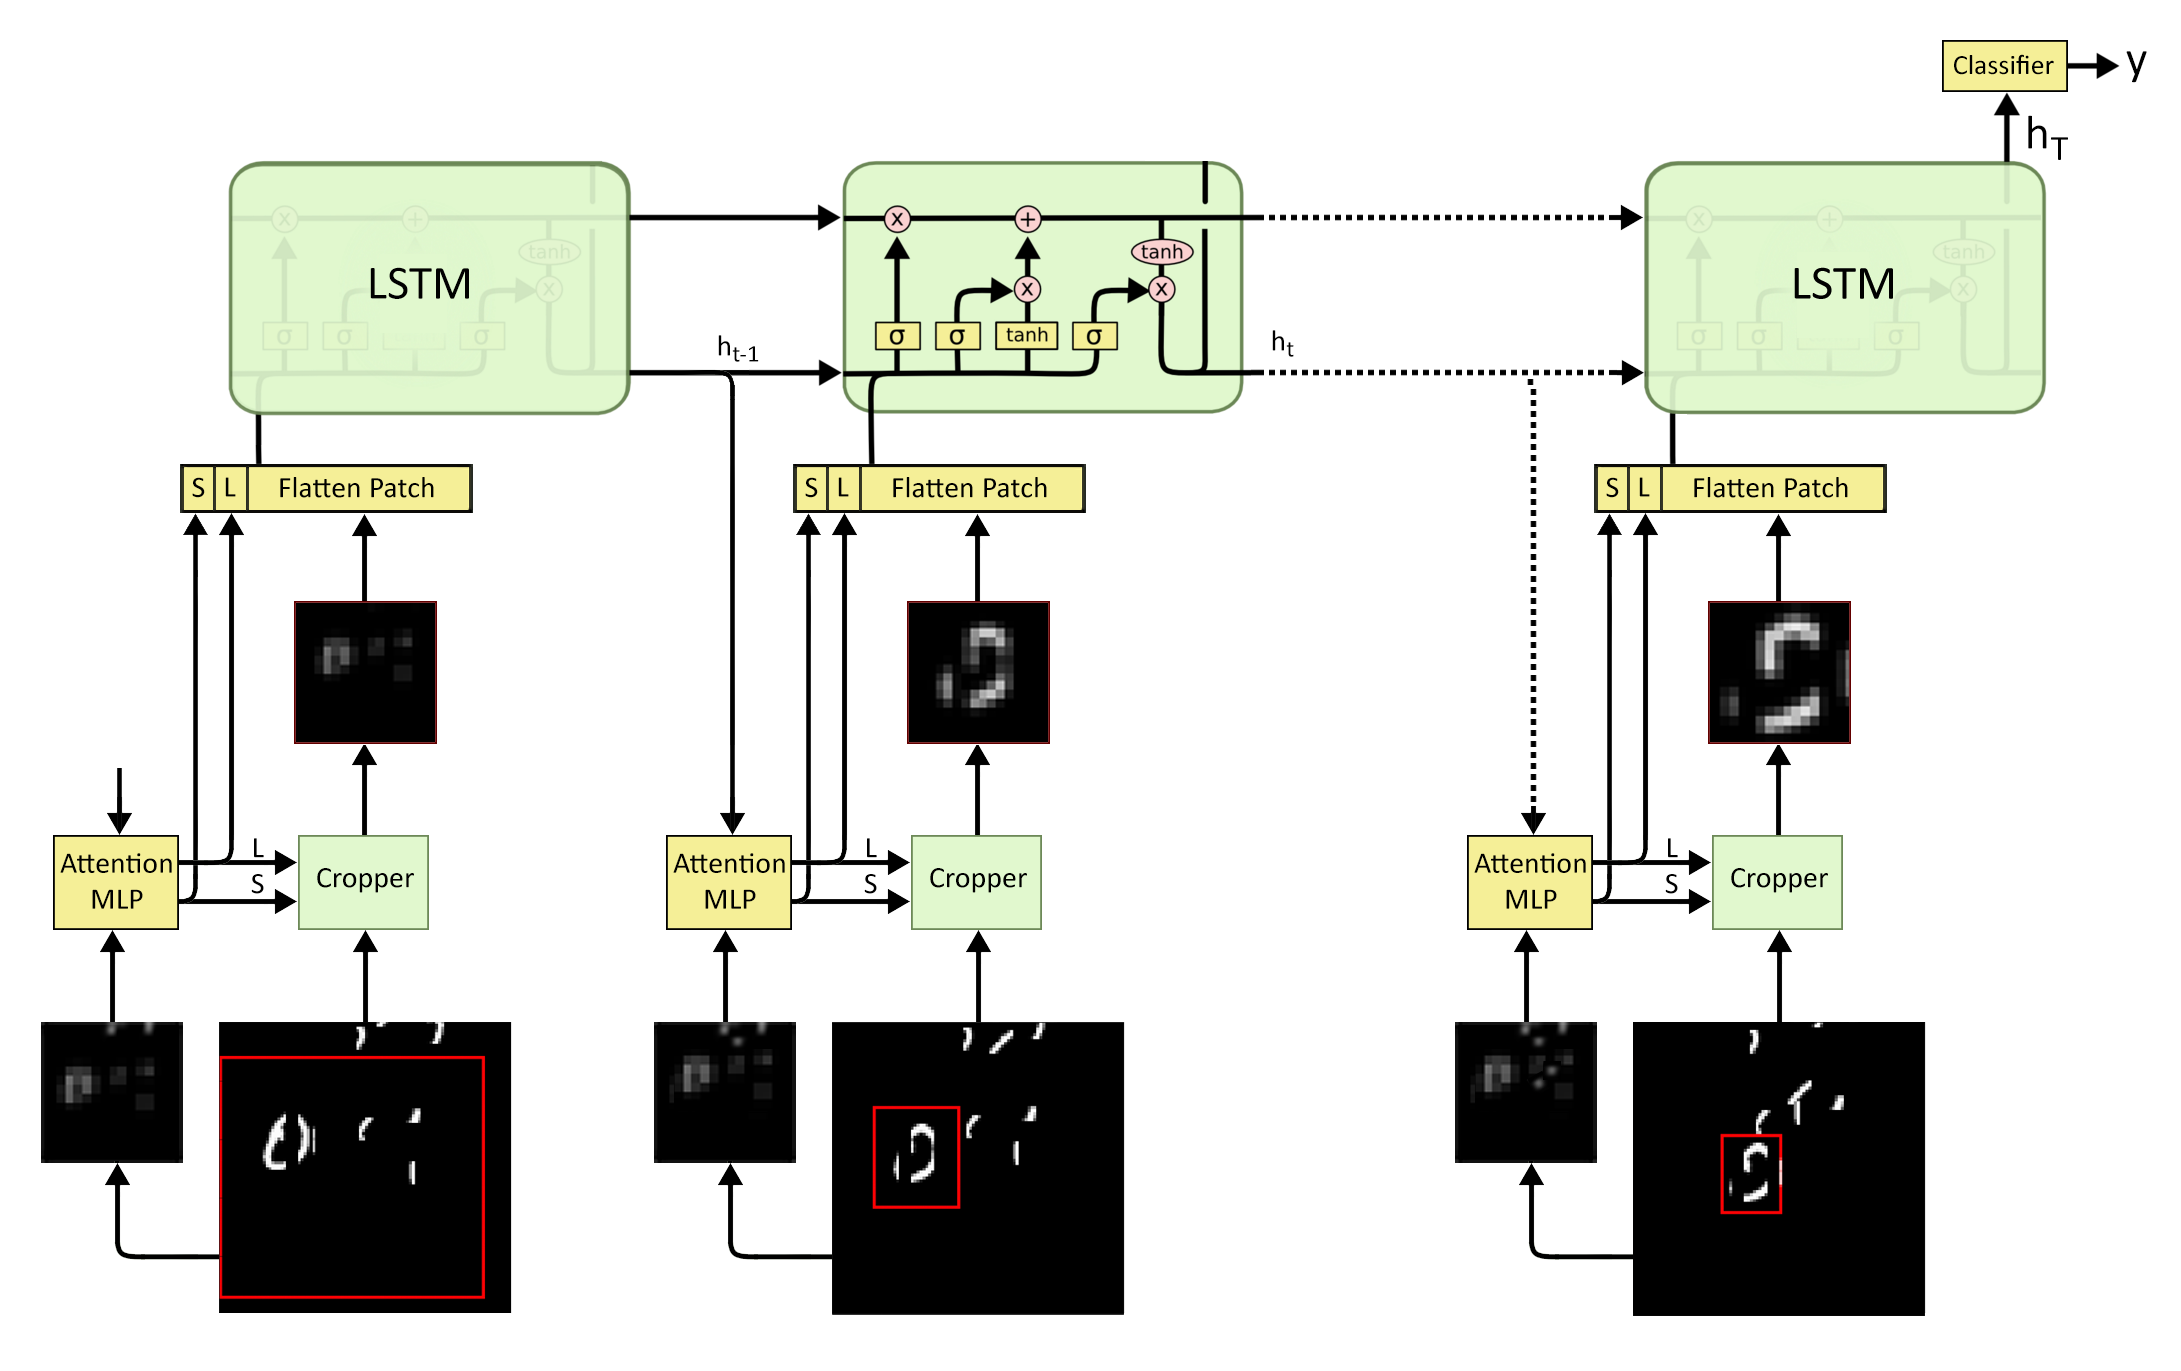
\includegraphics[width=17cm, height=12cm]{LSTM_2D_Attention_v2.png}
\section{Three-dimensional attention}

Our model processes a video $V$ through a sequence of three-dimensional glimpses $\left(v^{(t)}\right)$.
A glimpse corresponds to a three-dimensional hyper-rectangular volume of video defined by location and scale parameters $\theta^{(t)}$, resampled to a representation of constant size much smaller than the original video.
The resampling process is described in \ref{sec:resampling}.

Each resampled glimpse $v^{(t)}$ is passed through a convolutional network, concatenated with its parameters $\theta^{(t)}$ and fed to a fully-connected network to obtain the input $x^{(t)}$ to the next step of the recurrent network.

We use a two-layer recurrent neural network with Gated Recurrent Units\cite{Cho2014} to combine the information from previous glimpses and determine the location and scale of the next glimpse.

Figure \ref{fig:model} shows a schematic view of the model.

\includegraphics[width=10cm, height=12cm]{3D}


\include{threedfigure}

\section{Resampling}
\label{sec:resampling}

We employ a differential cropping operator similar to that used in DRAW \cite{draw}.
It is explained here for the three-dimensional case in which the input is
a video, but the application to two-dimensional video frames is similar.
The intensity of each pixel in the glimpse is a linear combination of the intensities of all the pixels in the video, with coefficients determined by Gaussian kernels.
The kernel covariance is constrained to be diagonal, which allows to resample across each of the temporal, vertical and horizontal data dimensions independently.
In the one-dimensional case, glimpse pixels $v_i$ relate to video pixels $V_i$ by

\begin{equation}
\begin{split}
v_i &= \sum_{\tilde{i}} \phi(\delta,\sigma) V_{\tilde{i}} \\
\delta & =  \frac{i - m/2}{s} + l - \tilde{i} \\
\sigma & =  \frac{\alpha}{\min(s, 1)}
\end{split}
\end{equation}

where $i$ is a glimpse pixel index, $\tilde{i}$ is a video pixel index, $m$ is the size of the glimpse in pixels, and $l$ and $s$ are the location and scale of the glimpse, respectively.
$\phi( \delta, \sigma ) = \frac{1}{\sqrt{2 \pi}\sigma} \exp{- \frac{1}{2} \frac{\delta^2}{\sigma^2}}$ is the Gaussian filter.

Note that the kernel stride, standard deviation and intensity scaling factor are determined by a single scale parameter $s$.
Disconnecting these parameters as is done in \cite{draw} would give the model the freedom to introduce severe resampling artifacts such as aliasing, unnecessary blurring and noise.
The influence of $s$ on $\sigma$ is bounded to avoid too narrow kernels when zooming in beyond the native resolution of the input.
The hyperparameter $\alpha$ trades off aliasing and blurring; by visual inspection of the quality of the patches we chose to set it to $0.5$.

We further depart from \cite{draw} by truncating the Gaussian kernels at three deviations from their means.
In practice we implement this by projecting the corners of the glimpse into the space of video indices and cropping a box around them with the desired margin.
The outermost kernels are thus more truncated than the interior ones, and the pixels in the center of the glimpse are virtually untruncated.
The resulting equations are still differentiable, with the gradient providing information on where to move inside the box.
We have found this truncation to have little effect on training, while allowing significant computational savings.

\section{Datasets}
\subsection{CMV: Cluttered MNIST Videos}

We introduce a new fine-grained video classification dataset derived from the Cluttered MNIST dataset \cite{clutteredmnist}.
The examples consist of MNIST digits placed on a larger canvas in the presence of clutter.
Both the digit and the clutter move across the canvas over time according to identical motion models, in which we uniformly sample a time $t$ and a location $x$ for the object in the interior of the video and extrapolate a linear trajectory based on a uniformly chosen velocity.

Additionally, we partially occlude the digit by superimposing black bars perpendicular to its direction of travel.
This ensures that no one frame displays the entire digit, and thus solving the task requires aggregation of information over time.

With this dataset we intend to bridge the gap between datasets such as KTH \cite{kth} and UCF101 \cite{ucf101} that have too few examples for the kinds of architectures we are interested in and large datasets like Sports-1M \cite{sports1m} and LSMDC \cite{lsmdc} that are too expensive to experiment on.

\subsection{Modified MPII cooking2 dataset}
\textbf{should be modified} The recent MPII cooking2 dataset is designed for the challenging task of fine-grained action recognition. 30 human subjects perform a large number of realistic cooking activities in 273 videos. Length of videos is over 27 hours. Most parts of the videos are annotated by an attribute among predefined 222 attributes. Attributes are 1. activities 2. tools 3. containers and 4. ingredients. The number of annotated samples is 14105. Each sample can have more than 1 label from different attribute categories. 
How do we modify the dataset and why do we need modification for training a deep network on this dataset? 
1) There are some samples that have only a few frames, and some which has over 5000 frames and only described by 1 attribute. As the first step of modification we remove the outliers from the dataset. Removing very short and long videos reduce the size of the dataset from 14105 to 8727.
2) To train a deep model we need to have enough samples from each attribute categories. However we only have a few samples for many classes. So in order to use only the attributes that have enough samples we just choose 10 attribute labels that have the maximum number of samples and remove the rest. At the end, we have a dataset of 8046 samples and 10 attributes.
\subsubsection*{Acknowledgments}

WRITEME

\bibliography{iclr2016_conference}
\bibliographystyle{iclr2016_conference}

\end{document}
